\chapter{Pengujian}

\section{Pengujian Perangkat Lunak BSIS}
Berdasarkan rancangan pada \ref{sec:rancangan_perangkat_lunak_bsis} telah dibuat sebuah perangkat lunak yang dapat melakukan identifikasi dari suatu gambar masukkan dengan menggunakan teknik BSIS. Perangkat lunak yang dibuat berbentuk aplikasi berbasis \textit{web} yang terbagi ke \textit{server} dan \textit{client}. Bagian \textit{server} dibuat dengan menggunakan \textit{framework} Flask di Python. \textit{Server} akan menerima \textit{request} HTTP dari \textit{client} dan melakukan identifikasi pada gambar masukkan dengan menggunakan parameter-parameter yang diberikan. Bagian \textit{client} dibuat dengan bentuk aplikasi \textit{web} berbasis React. Tampilan halaman \textit{client} saat aplikasi pertama dijalankan dapat dilihat pada Gambar~\ref{fig:client_1}.
\begin{figure}[H]
	\centering
	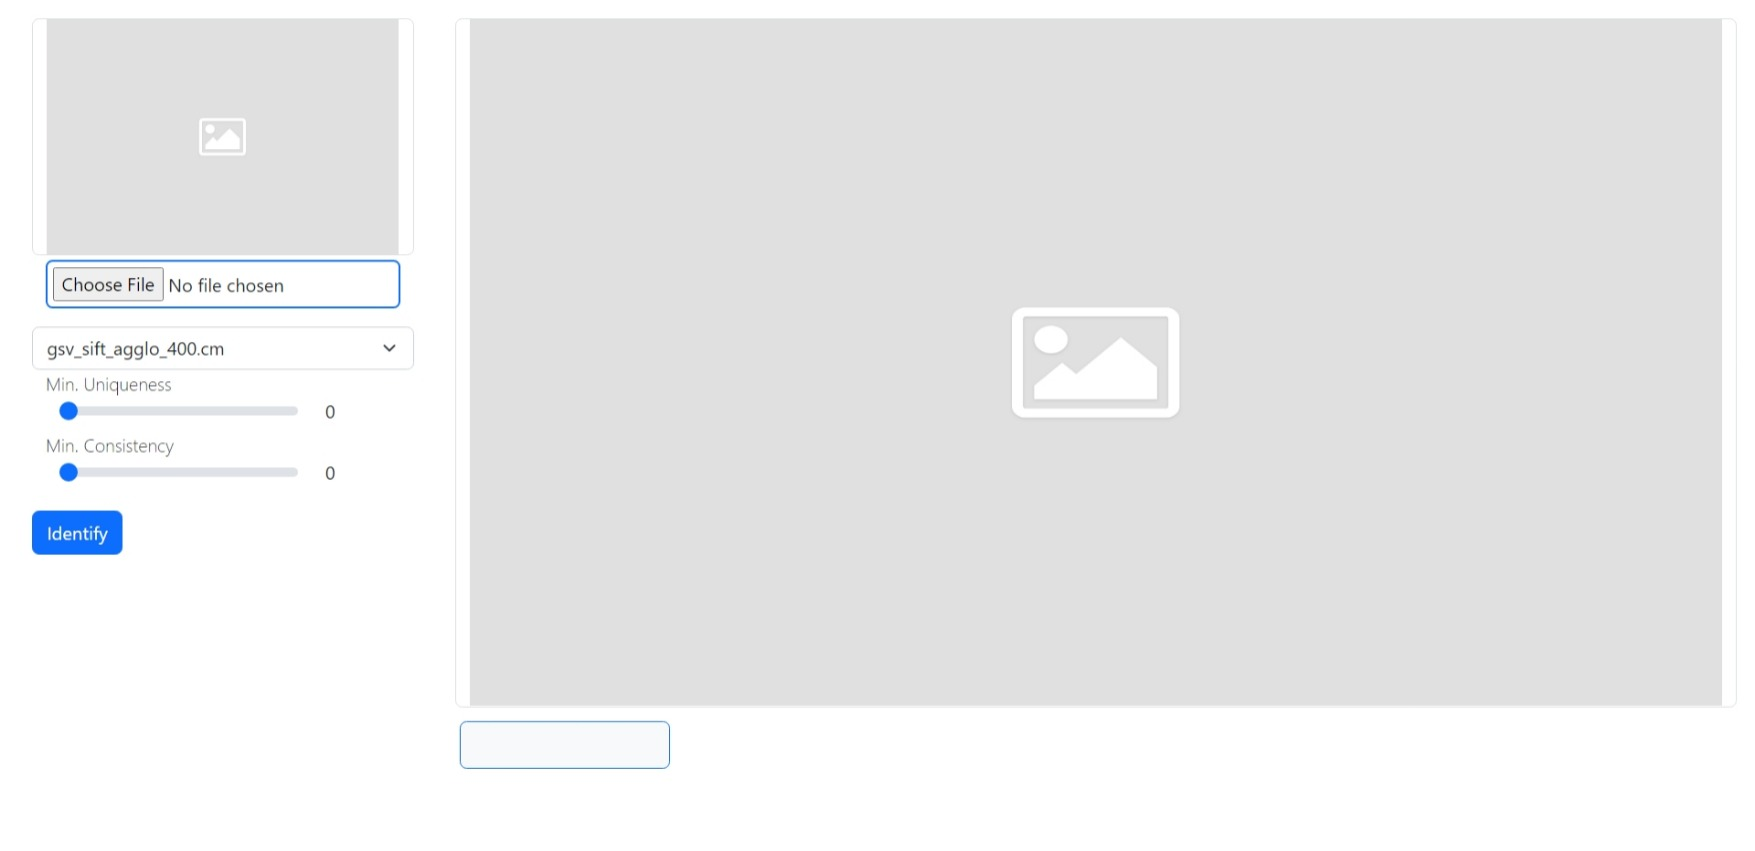
\includegraphics[width=\textwidth]{client_1.jpeg}
	\caption{Tampilan awal aplikasi perangkat lunak BSIS.}
	\label{fig:client_1}
\end{figure}

Pada bagian kiri halaman terdapat panel untuk \textit{input}. Bagian paling atas merupakan tempat untuk memilih gambar \textit{input}, saat tombol ``\textit{Choose file}'' ditekan akan membuka sebuah \textit{window} baru untuk memilih \textit{file} dari \textit{directory} lokal. Setelah dipilih gambar akan ditampilkan pada bagian kotak gambar. Tampilan aplikasi saat telah memilih gambar dapat dilihat pada Gambar~\ref{fig:client_2}. 
\begin{figure}[H]
	\centering
	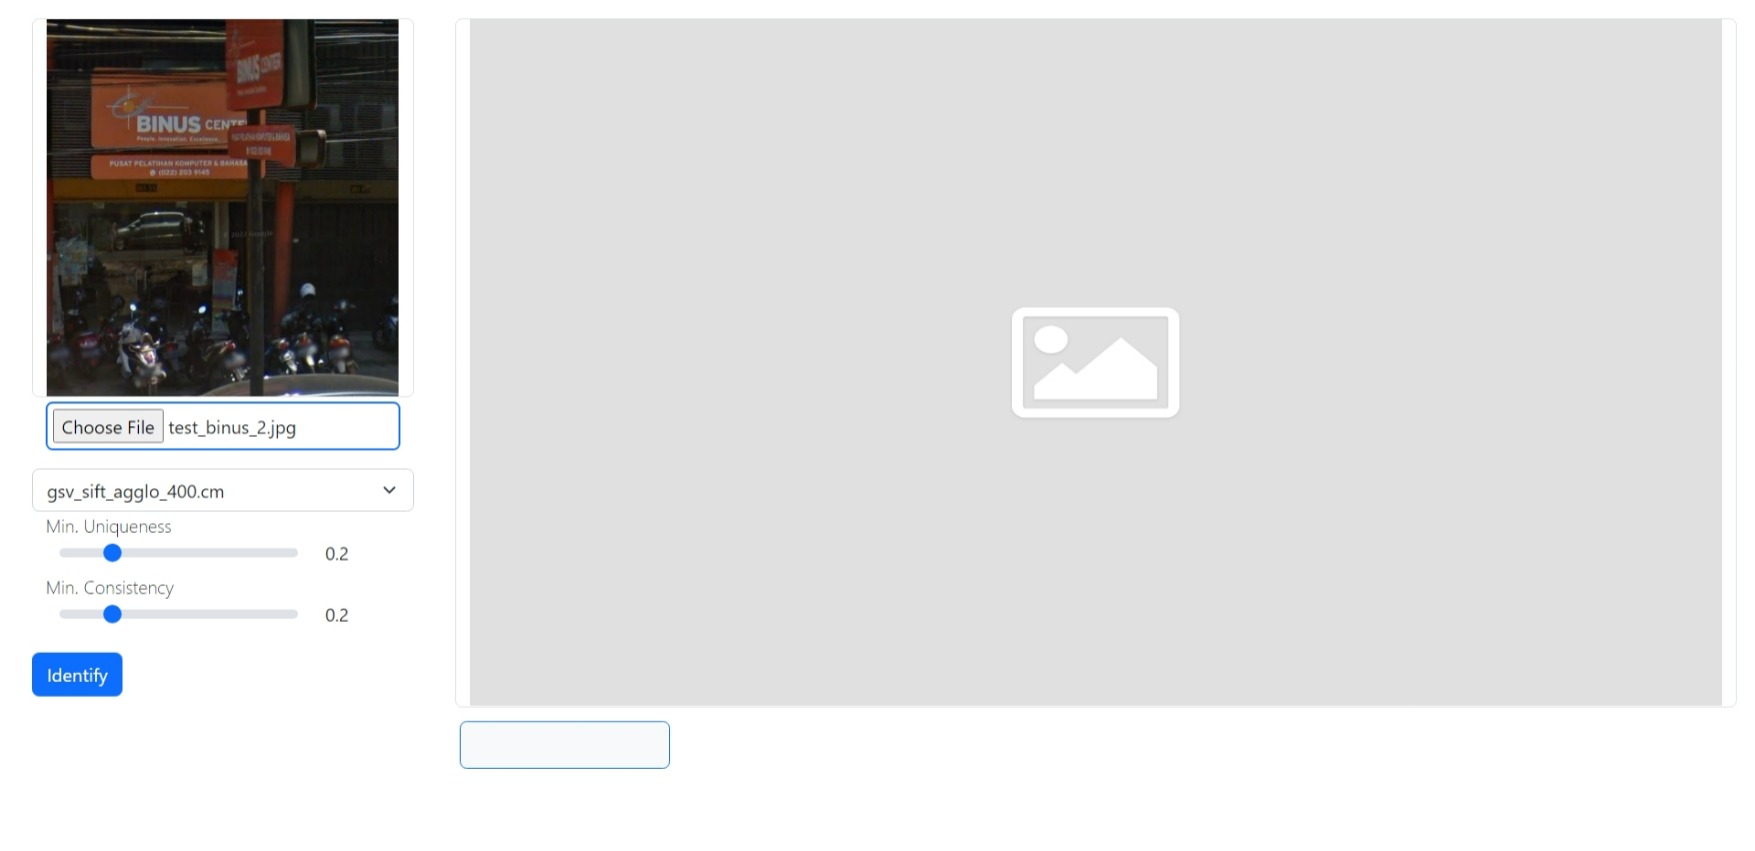
\includegraphics[width=\textwidth]{client_2.jpeg}
	\caption{Tampilan aplikasi perangkat lunak BSIS setelah memilih gambar \textit{input}.}
	\label{fig:client_2}
\end{figure}

Bagian di bawah tombol ``Choose file'' merupakan sebuah \textit{dropdown} yang berisi daftar model \texttt{ClusterModel} (lihat \ref{sec:clustermodel_class}) yang dapat digunakan. Di bawah \textit{dropdown} pemilihan model terdapat dua \textit{slider} yang berguna untuk menetukan \textit{threshold} untuk nilai konsistensi dan nilai keunikan. Setelah dipilih gambar \textit{input} dan model yang akan digunakan serta telah ditentukan \textit{threshold} untuk nilai konsistensi dan keunikan maka dapat dilakukan identifikasi dengan menekan tombol ``\textit{Identify}'' di bawah \textit{slider} nilai keunikan. Setelah ditekan tombol ``\textit{Identify}'' maka di bagian kanan akan ditampilkan hasil pemasangan \textit{keypoint} dari gambar \textit{input} dengan gambar di \textit{dataset} yang memiliki nilai total bobot dari BSIS paling tinggi. Tampilan aplikasi setelah dilakukan identifikasi pada gambar \textit{input} dapat dilihat pada Gambar~\ref{fig:client_3}.
\begin{figure}[H]
	\centering
	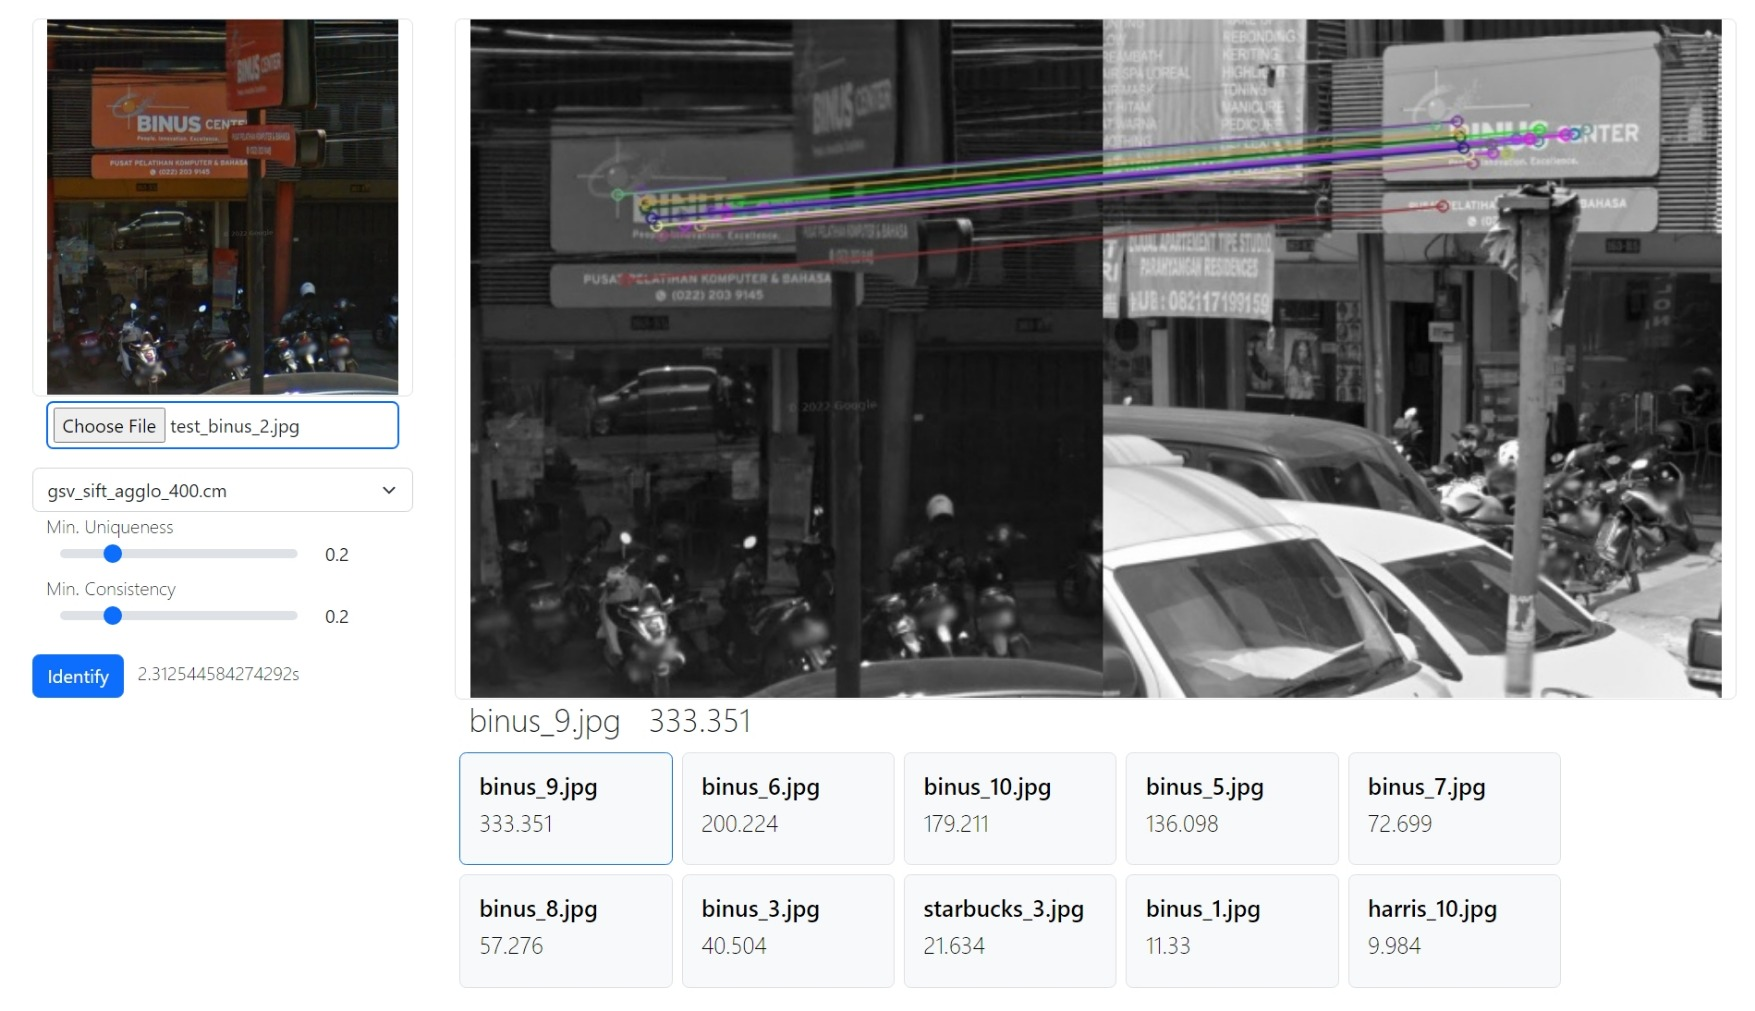
\includegraphics[width=\textwidth]{client_3.jpeg}
	\caption{Tampilan aplikasi perangkat lunak BSIS melakukan identifikasi pada gambar \textit{input}.}
	\label{fig:client_3}
\end{figure}
Pada bagian kanan halaman aplikasi---seperti yang dapat dilihat pada Gambar~\ref{fig:client_3}---terlihat gambar yang menunjukkan pemasangan \textit{keypoint} dari gambar \textit{input} dengan sebuah gambar \textit{dataset}. Pada bagian bawah gambar pemasangan \textit{keypoint} terdapat teks yang menunjukkan nama gambar dan disebelahnya merupakan total bobot pasangan gambar tersebut. Di bawah teks terdapat sebuah \textit{list} yang menunjukkan 10 gambar dari \textit{dataset} yang memiliki nilai total bobot BSIS tertinggi. Setiap \textit{item} dalam \textit{list} dapat ditekan untuk menampilkan pasangan \textit{keypoint} dengan gambar tersebut.

\section{Pengujian Metode Clustering untuk Identifikasi dengan BSIS}
Pada bab ini akan dilakukan pengujian untuk melihat efek penerapan metode \textit{clustering} untuk menyaring fitur lokal terhadap ketepatan dan waktu proses BSIS. Pengujian yang dilakukan ini akan menggunakan cara yang sama dengan yang ada pada \ref{sec:analisis_bsis} tetapi dengan menggunakan \textit{dataset} dan parameter \textit{threshold} yang berbeda. Pada pengujian ini akan digunakan \textit{dataset} GSV (\ref{subsec:dataset_gsv}).

\subsection{Ide Analisis}
Seperti yang telah dijelaskan sebelumnya, pengujian yang dilakukan pada bagian ini akan mengikuti alur yang telah dilakukan sebelumnya pada \ref{sec:analisis_bsis}. Pengujian ini bertujuan untuk menguji bagaimana penyaringan fitur lokal berdasarkan nilai konsistensi dan keunikannya dapat berpengaruh terhadap hasil saat dilakukan identifikasi terhadap gambar. Pengaruh hasil identifikasi yang diamati merupakan bagaimana tingkat akurasi dan waktu proses yang diperlukan untuk melakukan identifikasi.

Pada pengujian ini penyaringan fitur lokal akan dilakukan menggunakan dua cara. Penyaringan pertama dilakukan dengan menggunakan nilai \textit{threshold} yang didapat dari hasil analisis di \ref{sec:analisis_threshold}. Berdasarkan pada hasil analisis di \ref{sec:analisis_threshold}, penyaringan pertama akan dilakukan dengan menggunakan nilai \textit{threshold} 0.6 untuk konsistensi dan 0.7 untuk keunikan. Penyaringan kedua ditujukan untuk menggunakan nilai \textit{threshold} yang lebih rendah sehingga dapat digunakan sebagai perbandingan. Untuk penyaringan kedua akan ditentukan \textit{threshold} dengan cara yang sama dengan penentuan \textit{threshold} pada analisis di \ref{sec:analisis_threshold}. 

Pengujian ini akan dilakukan menggunakan \textit{dataset} GSV dengan dua ukuran gambar yang berbeda sama seperti pada analisis di \ref{sec:analisis_bsis}. Dua ukuran gambar yang digunakan akan dinamakan GSV 400 dan GSV 600, sesuai ukuran sisi terpanjang pada gambar-gambar yang digunakan. Berbeda dengan analisis pada \ref{sec:analisis_bsis}, pada pengujian ini ukuran dari gambar di data \textit{test} akan disesuaikan dengan ukuran gambar yang digunakan pada \textit{dataset}. Pengujian juga akan dilakukan dengan menggunakan dua metode ekstraksi fitur lokal yaitu SIFT dan ORB.

\subsection{Penentuan Threshold dan Hasil Analisis Metode SIFT}
\subsubsection{GSV 400}
Sebaran nilai konsistensi dan keunikan untuk \textit{dataset} GSV 400 dapat dilihat pada Gambar~\ref{fig:consistency_gsv400_pengujian_sift} dan Gambar~\ref{fig:uniqueness_gsv400_pengujian_sift}.
\begin{figure}[H]
	\centering
	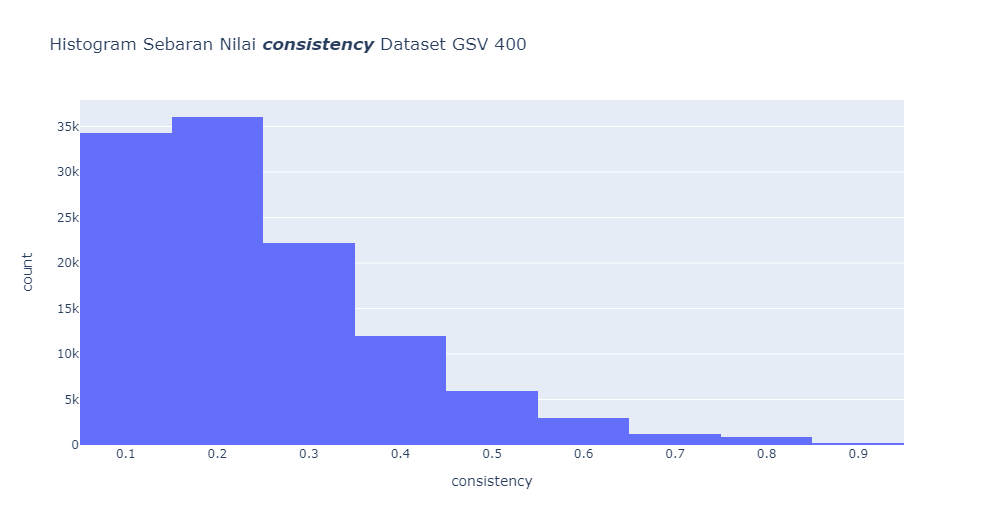
\includegraphics[width=\textwidth]{consistency_gsv400.png}
	\caption{Histogram sebaran nilai keunikan pada \textit{dataset} GSV 400.}
	\label{fig:consistency_gsv400_pengujian_sift}
\end{figure}

\begin{figure}[H]
	\centering
	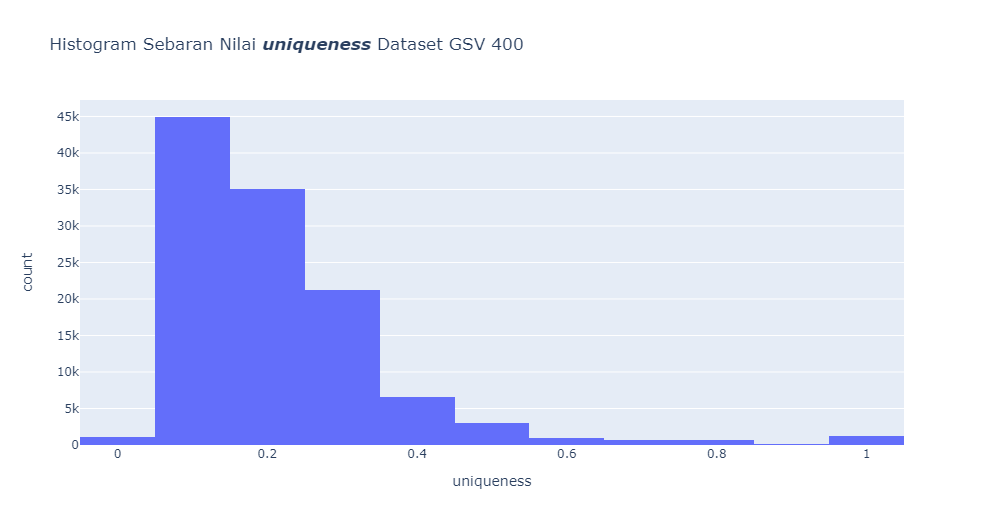
\includegraphics[width=\textwidth]{uniqueness_gsv400.png}
	\caption{Histogram sebaran nilai keunikan \textit{dataset} GSV 400.}
	\label{fig:uniqueness_gsv400_pengujian_sift}
\end{figure}
Dengan melihat sebaran nilai konsistensi dan keunikan pada Gambar~\ref{fig:consistency_gsv400_pengujian_sift} dan Gambar~\ref{fig:uniqueness_gsv400_pengujian_sift} maka akan digunakan nilai \textit{threshold} senilai 0.3 untuk konsistensi dan 0.3 untuk keunikan. Kedua nilai tersebut didapat dengan cara yang sama dengan yang dilakukan pada \ref{sec:analisis_bsis}. 

Pengujian pada \textit{dataset} GSV 400 akan dilakukan dengan menggunakan 3 set \textit{threshold} yang berbeda. Ketiga set \textit{threshold} yang digunakan dapat dilihat pada Tabel~\ref{tab:threshold_gsv400_sift}.
\begin{table}[H]
	\centering
	\begin{tabular}{|l|l|l|}
		\hline
		& \textbf{Konsistensi} & \textbf{Keunikan} \\ \hline
		\textbf{Keseluruhan} & 0.0                  & 0.0               \\ \hline
		\textbf{Threshold 1} & 0.3                  & 0.3               \\ \hline
		\textbf{Threshold 2} & 0.6                  & 0.7               \\ \hline
	\end{tabular}
	\caption{Tiga set \textit{threshold} yang digunakan untuk metode SIFT \textit{dataset} GSV 400.}
	\label{tab:threshold_gsv400_sift}
\end{table}
Hasil dari pengujian dapat dilihat pada Tabel~\ref{tab:pengujian_sift_gsv400}. Untuk sebaran waktu bagi tiap nilai \textit{threshold} yang digunakan dapat dilihat pada \textit{boxplot} di Gambar~\ref{fig:waktu_pengujian_sift_gsv400}.
\begin{table}[H]
	\centering
	\begin{tabular}{|l|l|l|l|}
		\hline
		& \textbf{Total Waktu Ekstraksi (s)} & \textbf{Total Waktu BSIS(s)} & \textbf{Akurasi (\%)} \\ \hline
		Keseluruhan & 1.29	&	92.55                    & 94                    \\ \hline
		Threshold 1 & 1.23	&	24.09                    & 84                    \\ \hline
		Threshold 2 & 1.23	&	13.97                    & 12                    \\ \hline
	\end{tabular}
	\caption{Hasil pengujian pada \textit{dataset} GSV 400.}
	\label{tab:pengujian_sift_gsv400}
\end{table}
\begin{figure}[H]
	\centering
	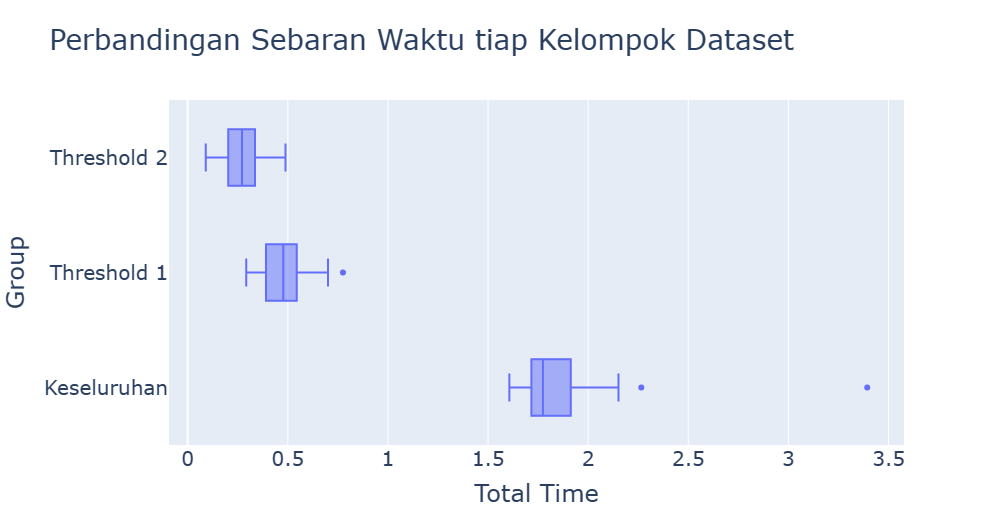
\includegraphics[width=\textwidth]{waktu_pengujian_sift_gsv400.png}
	\caption{Sebaran waktu pengujian metode SIFT \textit{dataset} GSV 400.}
	\label{fig:waktu_pengujian_sift_gsv400}
\end{figure}

Dari \textit{boxplot} pada Gambar~\ref{fig:waktu_pengujian_sift_gsv400} terlihat bahwa terdapat perbedaan sebaran waktu yang cukup signifikan antara \textit{dataset} keseluruhan dan \textit{dataset} yang tersaring. Perbedaan cukup tinggi terlihat di antara \textit{dataset} Keseluruhan dan hasil penyaringan dengan Threshold 1, sedangkan untuk perbedaan antara penyaringan dengan Threshold 1 dan Threshold 2 perbedaannya tidak terlalu signifikan. Rincian nilai untuk ketiga \textit{boxplot} pada Gambar~\ref{fig:waktu_pengujian_sift_gsv600} dapat dilihat pada Tabel~\ref{tab:boxplot_gsv400_sift} berikut.
\begin{table}[H]
	\centering
	\begin{tabular}{|l|l|l|l|}
		\hline
		& \textbf{Keseluruhan} & \textbf{Threshold 1} & \textbf{Threshold 2} \\ \hline
		\textit{min}          & 1.6063 & 0.2920 & 0.0902              \\ \hline
		\textit{lower fence}  & 1.6063 & 0.2920 & 0.0902              \\ \hline
		q1                    & 1.1716 & 0.3915 & 0.2020              \\ \hline
		q2 (median)           & 1.7741 & 0.4778 & 0.2714              \\ \hline
		q3                    & 1.9132 & 0.5442 & 0.3365              \\ \hline
		\textit{upper fence}  & 2.1514 & 0.7007 & 0.4890              \\ \hline
		\textit{max}          & 3.3937 & 0.7756 & 0.4890              \\ \hline
	\end{tabular}
	\caption{Nilai-nilai perbandingan waktu metode SIFT \textit{dataset} GSV 400.}
	\label{tab:boxplot_gsv400_sift}
\end{table}

\subsubsection{GSV 600}
Sebaran nilai konsistensi dan keunikan untuk \textit{dataset} GSV 600 dapat dilihat pada Gambar~\ref{fig:consistency_gsv600_pengujian_sift} dan Gambar~\ref{fig:uniqueness_gsv600_pengujian_sift}.
\begin{figure}[H]
	\centering
	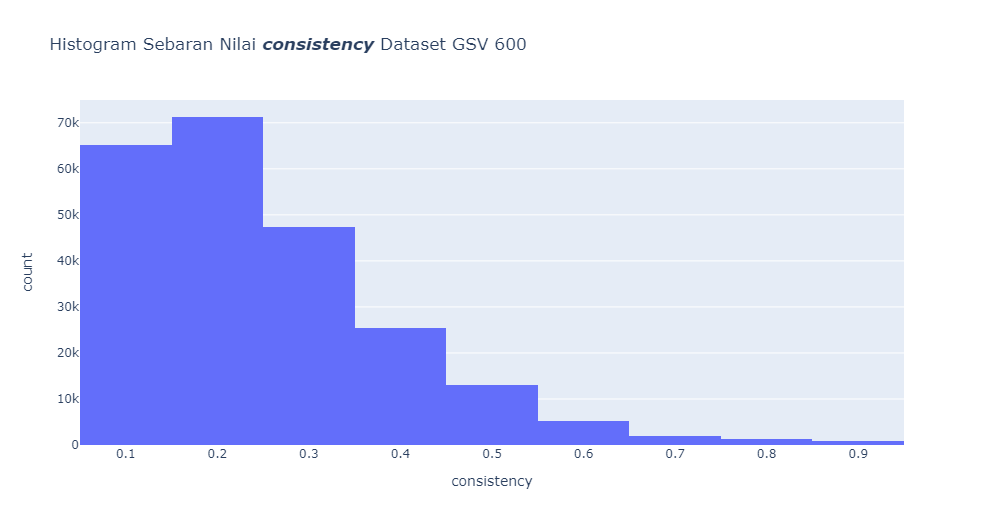
\includegraphics[width=\textwidth]{consistency_gsv600.png}
	\caption{Histogram sebaran nilai keunikan pada \textit{dataset} GSV 600.}
	\label{fig:consistency_gsv600_pengujian_sift}
\end{figure}

\begin{figure}[H]
	\centering
	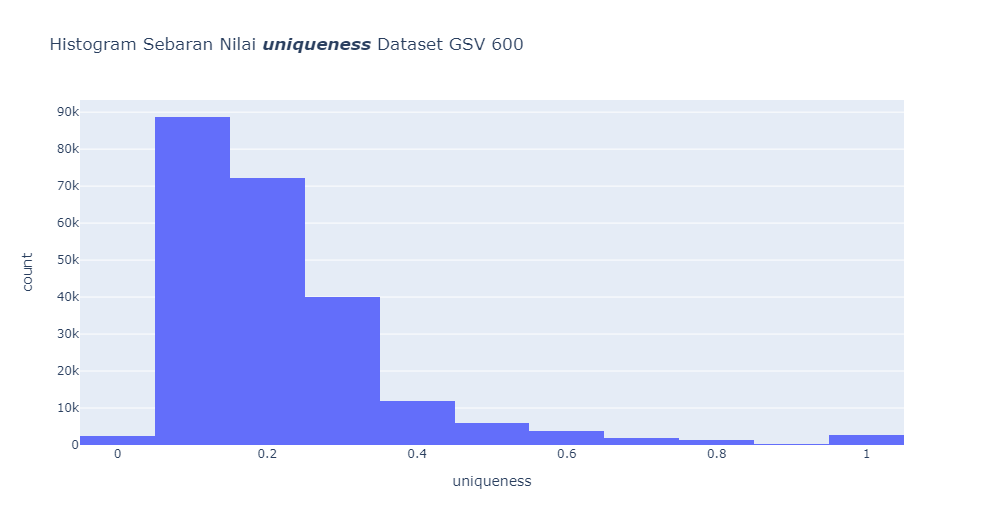
\includegraphics[width=\textwidth]{uniqueness_gsv600.png}
	\caption{Histogram sebaran nilai keunikan \textit{dataset} GSV 600.}
	\label{fig:uniqueness_gsv600_pengujian_sift}
\end{figure}
Dengan menggunakan cara yang sama seperti sebelumnya, berdasarkan sebaran yang dapat dilihat pada Gambar~\ref{fig:consistency_gsv600_pengujian_sift} dan Gambar~\ref{fig:uniqueness_gsv600_pengujian_sift} maka akan digunakan nilai \textit{threshold} senilai 0.3 untuk konsistensi dan 0.3 untuk keunikan. Tiga set \textit{threshold} yang digunakan pada pengujian \textit{dataset} ini dapat dilihat pada Tabel~\ref{tab:threshold_gsv600_sift}.
\begin{table}[H]
	\centering
	\begin{tabular}{|l|l|l|}
		\hline
		& \textbf{Konsistensi} & \textbf{Keunikan} \\ \hline
		\textbf{Keseluruhan} & 0.0                  & 0.0               \\ \hline
		\textbf{Threshold 1} & 0.3                  & 0.3               \\ \hline
		\textbf{Threshold 2} & 0.6                  & 0.7               \\ \hline
	\end{tabular}
	\caption{Tiga set \textit{threshold} yang digunakan untuk metode SIFT \textit{dataset} GSV 600.}
	\label{tab:threshold_gsv600_sift}
\end{table}
Setelah dilakukan pengujian terhadap \textit{dataset} GSV 600 dengan menggunakan tiga set \textit{threshold} tersebut didapat hasil yang dapat dilihat pada Tabel~\ref{tab:pengujian_sift_gsv600}. Sebaran waktu untuk tiap \textit{threshold} yang digunakan dapat dilihat secara rinci pada \textit{boxplot} di Gambar~\ref{fig:waktu_pengujian_sift_gsv600}.

\begin{table}[H]
	\centering
	\begin{tabular}{|l|l|l|l|}
		\hline
		& \textbf{Total Waktu Ekstraksi (s)} & \textbf{Total Waktu BSIS(s)} & \textbf{Akurasi (\%)} \\ \hline
		Keseluruhan & 2.50 & 189.54                   & 100                    \\ \hline
		Threshold 1 & 2.65 & 47.95                    & 84                    \\ \hline
		Threshold 2 & 2.39 & 22.04                    & 10                    \\ \hline
	\end{tabular}
	\caption{Hasil pengujian pada \textit{dataset} GSV 600.}
	\label{tab:pengujian_sift_gsv600}
\end{table}
\begin{figure}[H]
	\centering
	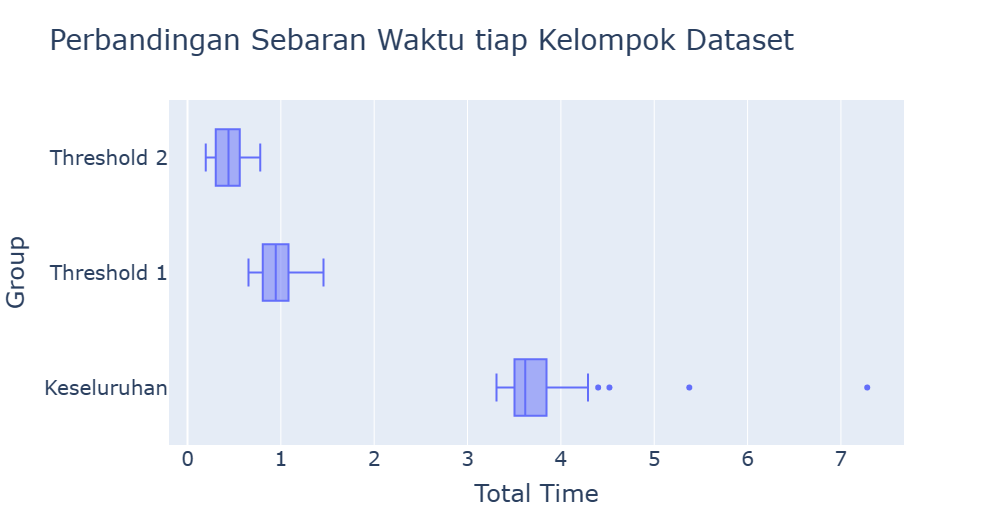
\includegraphics[width=\textwidth]{waktu_pengujian_sift_gsv600.png}
	\caption{Sebaran waktu pengujian metode SIFT \textit{dataset} GSV 600.}
	\label{fig:waktu_pengujian_sift_gsv600}
\end{figure}

Tiga buah \textit{boxplot} pada Gambar~\ref{fig:waktu_pengujian_sift_gsv600} menunjukkan perbedaan sebaran waktu antar tiga jenis \textit{dataset}. Seabran waktu di ketiga jenis \textit{dataset} tersebut relatif sama dengan sebaran pada saat digunakan \textit{dataset} GSV 400 (Gambar~\ref{fig:waktu_pengujian_sift_gsv400}). Terdapat perbedaan yang cukup signifikan antara \textit{dataset} keseluruhan dan yang telah tersaring dengan Threshold 1, tetapi untuk penyaringan Threshold 1 dan Threshold 2 perbedaannya tidak signifikan. Rincian nilai untuk ketiga \textit{boxplot} pada Gambar~\ref{fig:waktu_pengujian_sift_gsv600} dapat dilihat pada Tabel~\ref{tab:boxplot_gsv600_sift} berikut.
\begin{table}[H]
	\centering
	\begin{tabular}{|l|l|l|l|}
		\hline
		& \textbf{Keseluruhan} & \textbf{Threshold 1} & \textbf{Threshold 2} \\ \hline
		\textit{min}          & 3.3089 & 0.6535 & 0.1954              \\ \hline
		\textit{lower fence}  & 3.3089 & 0.6535 & 0.1954              \\ \hline
		q1                    & 3.5025 & 0.8086 & 0.3019              \\ \hline
		q2 (median)           & 3.6173 & 0.9444 & 0.4393              \\ \hline
		q3                    & 3.8465 & 1.0810 & 0.5591              \\ \hline
		\textit{upper fence}  & 4.2913 & 1.4579 & 0.7784              \\ \hline
		\textit{max}          & 7.2820 & 1.4579 & 0.7784              \\ \hline
	\end{tabular}
	\caption{Nilai-nilai perbandingan waktu metode SIFT \textit{dataset} GSV 600.}
	\label{tab:boxplot_gsv600_sift}
\end{table}

Hasil pada Tabel~\ref{tab:pengujian_sift_gsv400} dan Tabel~\ref{tab:pengujian_sift_gsv600} menunjukkan nilai \textit{threshold} yang didapat dari hasil analisis pada \textit{threshold} (\ref{sec:analisis_threshold}) memberikan hasil BSIS dengan akurasi yang sangat rendah. Cara penentuan \textit{threshold} dengan melihat hasil pada gambar tersebut ternyata tidak efektif jika digunakan untuk melakukan identifikasi. Hal ini mungkin dikarenakan dalam melakukan identifikasi gambar banyak fitur lokal yang berasal bukan dari bagian yang merupakan logo atau objek penting, tetapi sebenarnya berguna dalam identifikasi.

\subsection{Penentuan Threshold dan Hasil Analisis Metode ORB}
Pada pengujian dengan metode ORB ini hanya akan digunakan satu set \textit{threshold}. \textit{Threshold} yang digunakan adalah \textit{threshold} yang didapat dari melihat hasil sebaran nilai konsistensi dan keunikan. Nilai \texttt{threshold} yang didapat dengan melihat hasilnya pada gambar seperti pada \ref{sec:analisis_threshold} tidak digunakan pada pengujian ini, karena pada penelitian ini belum dilakukan analisis \textit{threshold} dengan menggunakan metode ORB. 

\subsubsection{GSV 400}
Sebaran nilai konsistensi dan keunikan untuk \textit{dataset} GSV 400 dapat dilihat pada Gambar~\ref{fig:consistency_gsv400_pengujian_orb} dan Gambar~\ref{fig:uniqueness_gsv400_pengujian_orb}.
\begin{figure}[H]
	\centering
	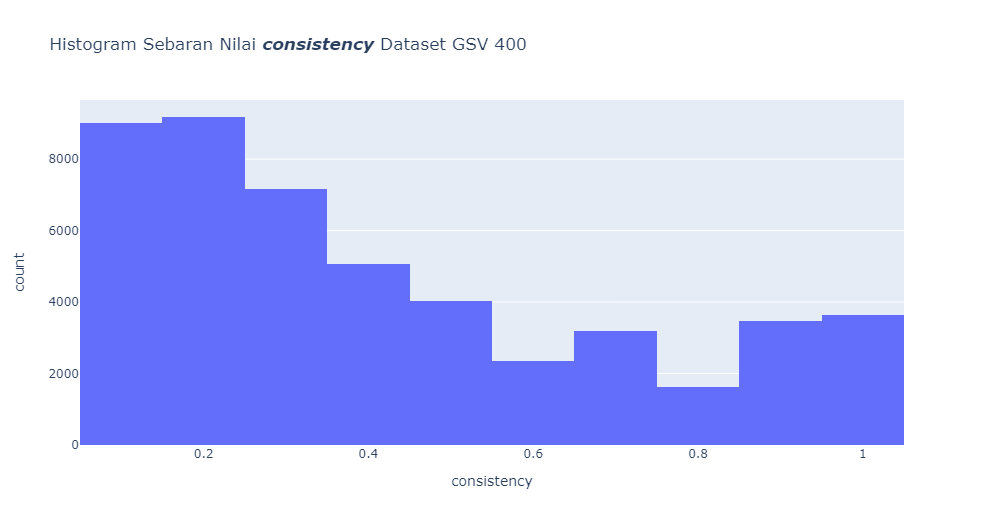
\includegraphics[width=\textwidth]{consistency_gsv400_orb.png}
	\caption{Histogram sebaran nilai keunikan pada \textit{dataset} GSV 400.}
	\label{fig:consistency_gsv400_pengujian_orb}
\end{figure}

\begin{figure}[H]
	\centering
	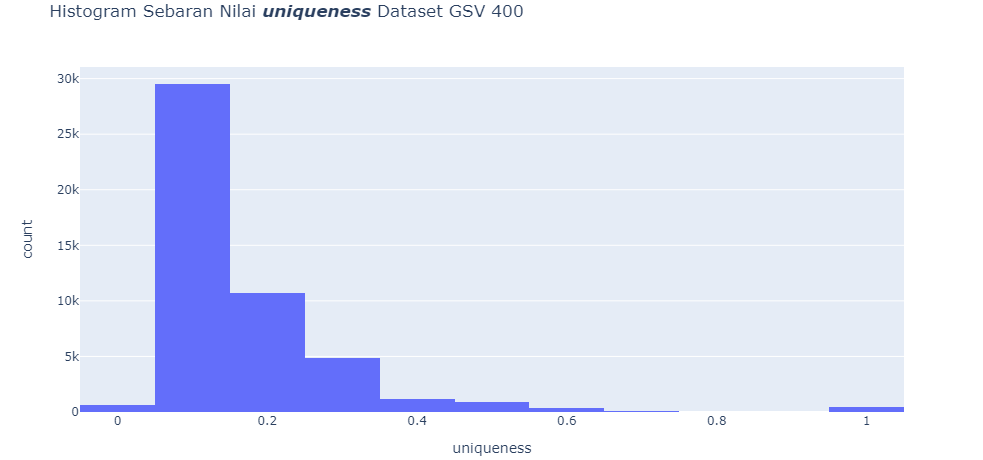
\includegraphics[width=\textwidth]{uniqueness_gsv400_orb.png}
	\caption{Histogram sebaran nilai keunikan \textit{dataset} GSV 400.}
	\label{fig:uniqueness_gsv400_pengujian_orb}
\end{figure}
Dari kedua histogram pada Gambar~\ref{fig:consistency_gsv400_pengujian_orb} dan Gambar~\ref{fig:uniqueness_gsv400_pengujian_orb} ditetapkan nilai \textit{threshold} untuk konsistensi senilai 0.3 dan untuk keunikan senilai 0.3. Dua set \textit{threshold} yang digunakan pada pengujian ini dapat dilihat pada Tabel~\ref{tab:threshold_gsv400_orb}.
\begin{table}[H]
	\centering
	\begin{tabular}{|l|l|l|}
		\hline
		& \textbf{Konsistensi} & \textbf{Keunikan} \\ \hline
		\textbf{Keseluruhan} & 0.0                  & 0.0               \\ \hline
		\textbf{Threshold 1} & 0.3                  & 0.3               \\ \hline
	\end{tabular}
	\caption{Tiga set \textit{threshold} yang digunakan untuk metode ORB \textit{dataset} GSV 400.}
	\label{tab:threshold_gsv400_orb}
\end{table}
Setelah dilakukan pengujian terhadap \textit{dataset} didapat hasil seperti yang dapat dilihat pada Tabel~\ref{tab:pengujian_orb_gsv400}. Untuk sebaran waktu secara rinci dapat dilihat pada \textit{boxplot} di Gambar~\ref{fig:waktu_pengujian_orb_gsv400}.
\begin{table}[H]
	\centering
	\begin{tabular}{|l|l|l|l|}
		\hline
		& \textbf{Total Waktu Ekstraksi (s)} & \textbf{Total Waktu BSIS(s)} & \textbf{Akurasi (\%)} \\ \hline
		Keseluruhan & 0.17 & 49.04                   & 78                    \\ \hline
		Threshold 1 & 0.17 & 2.08                    & 14                    \\ \hline
	\end{tabular}
	\caption{Hasil pengujian pada \textit{dataset} GSV 400.}
	\label{tab:pengujian_orb_gsv400}
\end{table}
\begin{figure}[H]
	\centering
	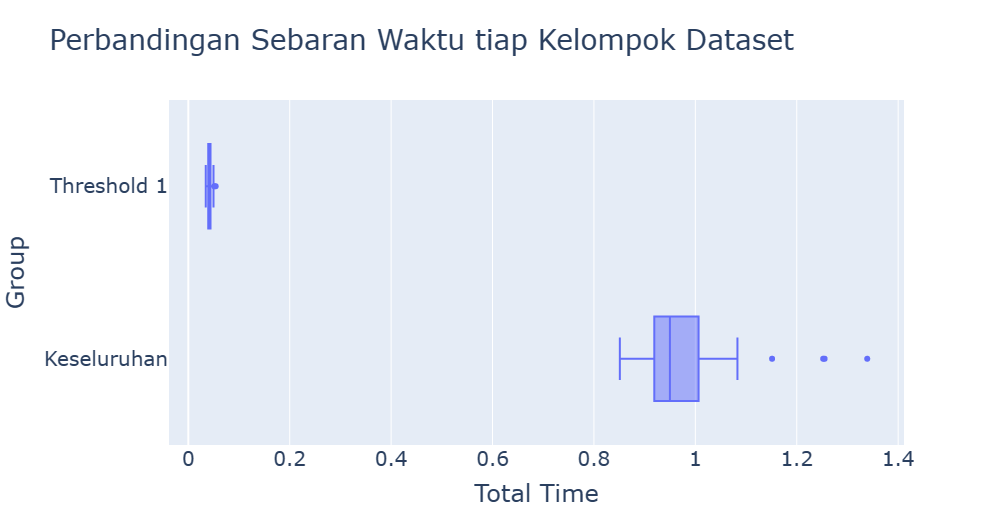
\includegraphics[width=\textwidth]{waktu_pengujian_orb_gsv400.png}
	\caption{Sebaran waktu pengujian metode ORB \textit{dataset} GSV 400.}
	\label{fig:waktu_pengujian_orb_gsv400}
\end{figure}

\textit{Boxplot} pada Gambar~\ref{fig:waktu_pengujian_orb_gsv400} menunjukkan perbedaan sebaran waktu antara \textit{dataset} GSV 400 secara keseluruhan dan yang telah tersaring dengan menggunakan Threshold 1. Jika dilihat terdapat perbedaan yang signifikan antar keduanya, nilai-nilai pada \textit{dataset} keseluruhan tersebar di kisaran 0.8 sampai 1.1, sedangkan untuk \textit{dataset} yang telah tersaring nilai-nilainya tersebar di kisaran 0.03 sampai 0.05. Rincian nilai untuk kedua \textit{boxplot} pada Gambar~\ref{fig:waktu_pengujian_orb_gsv400} dapat dilihat pada Tabel~\ref{tab:boxplot_gsv400_orb} berikut.
\begin{table}[H]
	\centering
	\begin{tabular}{|l|l|l|}
		\hline
		& \textbf{Keseluruhan} & \textbf{Threshold 1}         \\ \hline
		\textit{min}          & 0.8510 & 0.0344               \\ \hline
		\textit{lower fence}  & 0.8510 & 0.0344               \\ \hline
		q1                    & 0.9190 & 0.0391               \\ \hline
		q2 (median)           & 0.9498 & 0.0410               \\ \hline
		q3                    & 1.0063 & 0.0435               \\ \hline
		\textit{upper fence}  & 1.0829 & 0.0495               \\ \hline
		\textit{max}          & 1.3390 & 0.0540               \\ \hline
	\end{tabular}
	\caption{Nilai-nilai perbandingan waktu metode ORB \textit{dataset} GSV 400.}
	\label{tab:boxplot_gsv400_orb}
\end{table}


\subsubsection{GSV 600}
Sebaran nilai konsistensi dan keunikan untuk \textit{dataset} GSV 600 dapat dilihat pada Gambar~\ref{fig:consistency_gsv600_pengujian_orb} dan Gambar~\ref{fig:uniqueness_gsv600_pengujian_orb}.
\begin{figure}[H]
	\centering
	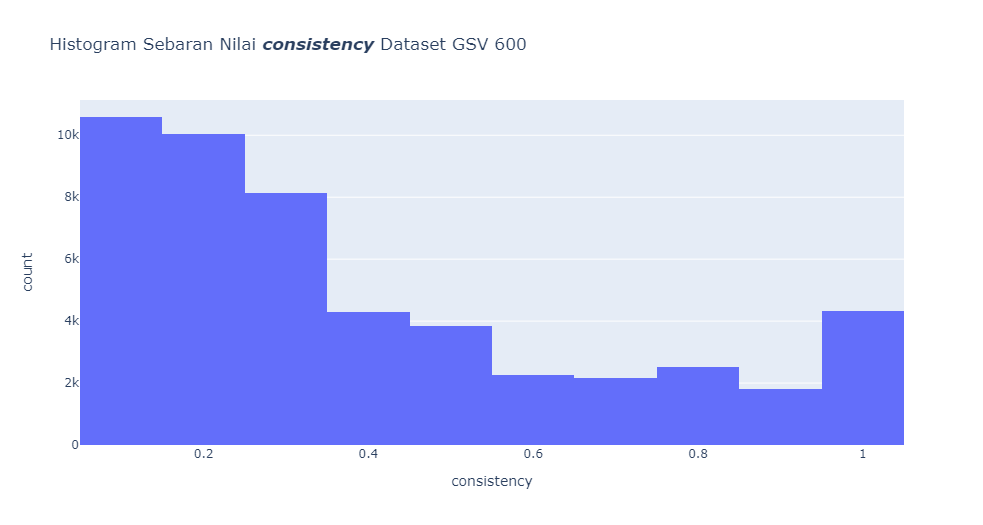
\includegraphics[width=\textwidth]{consistency_gsv600_orb.png}
	\caption{Histogram sebaran nilai keunikan pada \textit{dataset} GSV 600.}
	\label{fig:consistency_gsv600_pengujian_orb}
\end{figure}

\begin{figure}[H]
	\centering
	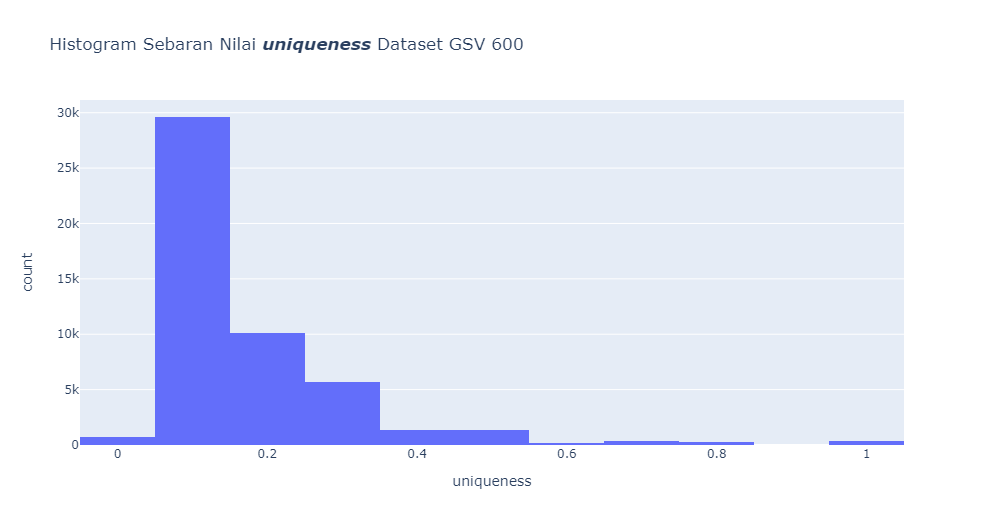
\includegraphics[width=\textwidth]{uniqueness_gsv600_orb.png}
	\caption{Histogram sebaran nilai keunikan \textit{dataset} GSV 600.}
	\label{fig:uniqueness_gsv600_pengujian_orb}
\end{figure}
Dapat dilihat dari kedua histogram di Gambar~\ref{fig:consistency_gsv600_pengujian_orb} dan Gambar~\ref{fig:uniqueness_gsv600_pengujian_orb} bahwa sebaran nilai konsistensi dan keunikan untuk GSV 600 sama dengan sebaran pada GSV 400. Dari sebaran nilai yang sama antara GSV 400 dan GSV 600 ini maka untuk GSV 600 dapat digunakan set \textit{threshold} yang sama dengan GSV 400. Dua set \textit{threshold} yang digunakan pada pengujian GSV 600 ini dapat dilihat pada Tabel~\ref{tab:threshold_gsv600_orb}.
\begin{table}[H]
	\centering
	\begin{tabular}{|l|l|l|}
		\hline
		& \textbf{Konsistensi} & \textbf{Keunikan} \\ \hline
		\textbf{Keseluruhan} & 0.0                  & 0.0               \\ \hline
		\textbf{Threshold 1} & 0.3                  & 0.3               \\ \hline
	\end{tabular}
	\caption{Tiga set \textit{threshold} yang digunakan untuk metode ORB \textit{dataset} GSV 600.}
	\label{tab:threshold_gsv600_orb}
\end{table}
Setelah dilakukan pengujian terhadap \textit{dataset} didapat hasil seperti yang dapat dilihat pada Tabel~\ref{tab:pengujian_orb_gsv600}. Waktu pengujian secara rinci dapat dilihat pada \textit{boxplot} di Gambar~\ref{fig:waktu_pengujian_orb_gsv600}. 
\begin{table}[H]
	\centering
	\begin{tabular}{|l|l|l|l|}
		\hline
		& \textbf{Total Waktu Ekstraksi (s)} & \textbf{Total Waktu BSIS(s)} & \textbf{Akurasi (\%)} \\ \hline
		Keseluruhan & 0.29 & 50.54                   & 80                    \\ \hline
		Threshold 1 & 0.29 & 2.92                    & 20                    \\ \hline
	\end{tabular}
	\caption{Hasil pengujian pada \textit{dataset} GSV 600.}
	\label{tab:pengujian_orb_gsv600}
\end{table}
\begin{figure}[H]
	\centering
	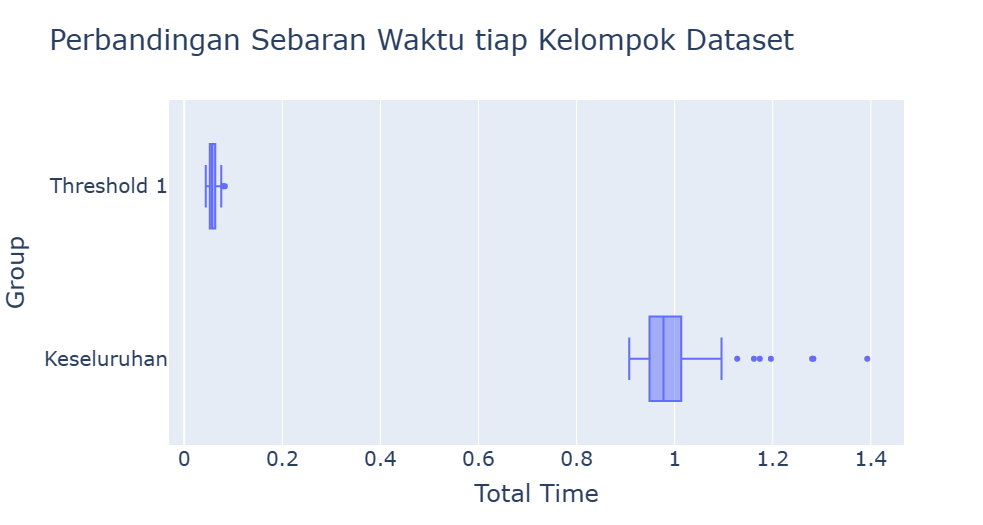
\includegraphics[width=\textwidth]{waktu_pengujian_orb_gsv600.png}
	\caption{Sebaran waktu pengujian metode ORB \textit{dataset} GSV 600.}
	\label{fig:waktu_pengujian_orb_gsv600}
\end{figure}

\textit{Boxplot} pada Gambar~\ref{fig:waktu_pengujian_orb_gsv600} menunjukkan perbedaan sebaran waktu antara \textit{dataset} GSV 600 secara keseluruhan dan yang sudah tersaring dengan Threshold 1. Secara garis besar perbedaan antar keduanya cukup signifikan, relatif sama dengan sebaran pada \textit{dataset} GSV 400 (Gambar~\ref{fig:waktu_pengujian_sift_gsv400}), hanya saja nilai-nilai pada \textit{dataset} GSV 600 berada pada kisaran nilai yang lebih tinggi. Pada \textit{dataset} GSV 600 ini secara keseluruhan nilai-nilainya berkisar di 0.9 sampai 1.1, sedangkan untuk yang telah tersaring nilai-nilainya berkisar di 0.04 sampai 0.07. Rincian nilai untuk kedua \textit{boxplot} pada Gambar~\ref{fig:waktu_pengujian_orb_gsv600} tersebut dapat dilihat pada Tabel~\ref{tab:boxplot_gsv600_orb} berikut.
\begin{table}[H]
	\centering
	\begin{tabular}{|l|l|l|}
		\hline
		& \textbf{Keseluruhan} & \textbf{Threshold 1}         \\ \hline
		\textit{min}          & 0.9073 & 0.0440               \\ \hline
		\textit{lower fence}  & 0.9073 & 0.0440               \\ \hline
		q1                    & 0.9487 & 0.0522               \\ \hline
		q2 (median)           & 0.9771 & 0.0567               \\ \hline
		q3                    & 1.0013 & 0.0631               \\ \hline
		\textit{upper fence}  & 1.0957 & 0.0758               \\ \hline
		\textit{max}          & 1.3927 & 0.0830               \\ \hline
	\end{tabular}
	\caption{Nilai-nilai perbandingan waktu metode ORB \textit{dataset} GSV 600.}
	\label{tab:boxplot_gsv600_orb}
\end{table}

\subsection{Analisis Hasil Pengujian}
Pada bagian analisis ini akan dibandingkan hasil dari pengujian antara SIFT dan ORB yang telah dilakukan. Pengujian yang dilakukan dengan menggunakan \textit{threshold} dari hasil analisis \textit{threshold} tidak akan ikut dibandingkan, karena nilai \textit{threshold} tersebut hanya digunakan pada pengujian dengan SIFT. Perbandingan yang dilakukan akan dibagi berdasarkan ukuran gambar yang digunakan. Hasilnya dapat dilihat pada subbab-subbab berikut ini.

\subsubsection{GSV 400}
\begin{table}[H]
	\centering
	\begin{tabular}{|p{.1\textwidth}|p{.15\textwidth}|p{.15\textwidth}|p{.15\textwidth}|p{.15\textwidth}|p{.15\textwidth}|}
		\hline
		&            & \textbf{Jumlah Fitur Lokal} & \textbf{Total Waktu Ekstraksi (s)} & \textbf{Total Waktu BSIS (s)} & \textbf{Akurasi (\%)} \\ \hline
		\multicolumn{1}{|l|}{\multirow{2}{*}{SIFT}} & Keseluruhan & 115685 & 1.25                            & 90.99                         & 94                    \\ \cline{2-6} 
		\multicolumn{1}{|l|}{}                      & Threshold 1 & 15365 & 1.29                            & 24.30                         & 84                    \\ \hline
		\multirow{2}{*}{ORB}                        & Keseluruhan & 48707 & 0.17                            & 51.12                         & 76                    \\ \cline{2-6} 
		& Threshold 1 & 1958 & 0.33                            & 1.81                          & 28                    \\ \hline
	\end{tabular}
	\caption{Hasil perbandingan pengujian SIFT dan ORB pada \textit{dataset} GSV 400.}
	\label{tab:perbandingan_gsv400}
\end{table}
Dari hasil pada Tabel~\ref{tab:perbandingan_gsv400} terlihat bahwa pada terdapat perbedaan hasil yang cukup signifikan antara SIFT dan ORB. Terlihat bahwa dari SIFT dan ORB terdapat penurunan waktu ekstraksi fitur yang cukup signifikan. Total waktu BSIS pada ORB juga menurun secara signifikan dibandingkan dengan SIFT, tetapi penurunan ini lebih dikarenakan jumlah fitur lokal yang dihasilkan ORB tidak sebanyak yang dihasilkan oleh SIFT. Nilai akurasi dari SIFT dan ORB juga mengalami penurunan yang signifikan. Akurasi dari ORB ada pada angka yang termasuk rendah terutama pada hasil yang telah disaring, hasil ini berbeda dari hasil yang didapat dari pengujian pada analisis di \ref{sec:analisis_orb}. Pada pengujian di analisis sebelumnya identifikasi dengan menggunakan metode ORB masih menghasilkan nilai akurasi yang cukup tinggi walaupun nilainya masih lebih kecil dari SIFT.

\subsubsection{GSV 600}
\begin{table}[H]
	\centering
	\begin{tabular}{|p{.1\textwidth}|p{.15\textwidth}|p{.15\textwidth}|p{.15\textwidth}|p{.15\textwidth}|p{.15\textwidth}|}
		\hline
		&             & \textbf{Jumlah Fitur Lokal} & \textbf{Total Waktu Ekstraksi (s)} & \textbf{Total Waktu BSIS (s)} & \textbf{Akurasi (\%)} \\ \hline
		\multicolumn{1}{|l|}{\multirow{2}{*}{SIFT}} & Keseluruhan & 231463 & 2.69                             & 187.64                        & 100                   \\ \cline{2-6} 
		\multicolumn{1}{|l|}{}                      & Threshold 1 & 33735 & 2.57                             & 47.58                         & 84                    \\ \hline
		\multirow{2}{*}{ORB}                        & Keseluruhan & 49968 & 0.31                             & 51.10                         & 78                    \\ \cline{2-6} 
		& Threshold 1 & 2145 & 0.29                             & 2.99                          & 20                    \\ \hline
	\end{tabular}
	\caption{Hasil perbandingan pengujian SIFT dan ORB pada \textit{dataset} GSV 600.}
	\label{tab:perbandingan_gsv600}
\end{table}
Hasil yang dapat dilihat pada Tabel~\ref{tab:perbandingan_gsv600} menunjukkan pola yang sama dari SIFT dan ORB, di mana SIFT memerlukan waktu yang lebih lama baik dari waktu ekstrak maupun waktu untuk BSIS, tetapi juga menghasilkan akurasi yang lebih tinggi. Pada \textit{dataset} ini waktu yang diperlukan baik untuk ekstrak maupun BSIS lebih tinggi dari waktu yang diperlukan \textit{dataset} GSV 400. Waktu yang lebih lama tersebut dikarenakan ukuran gambar yang lebih besar sehingga lebih banyak fitur lokal yang dapat dihasilkan dari tahap ekstraksi.


